\begin{figure*}[ht] 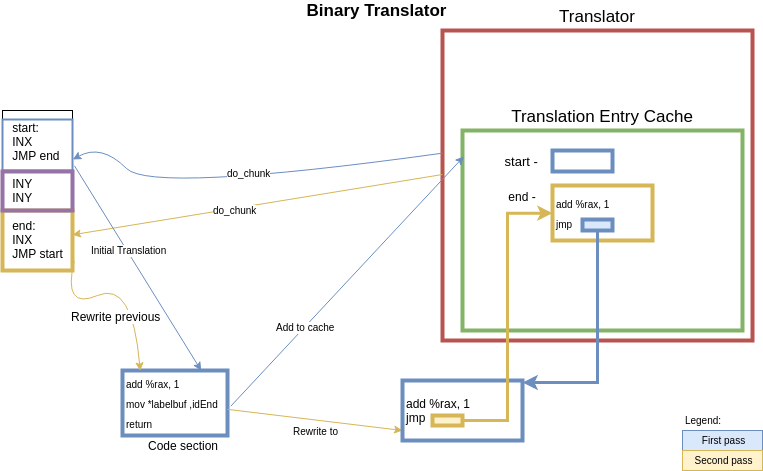
\includegraphics[width=\textwidth]{./images/translator.png}
\caption{The general overview of a simple binary translation} \label{fig:trans}
\end{figure*}

\section{A Better Design}

\subsection{Overview}

The general overview of a binary translator goes through the following steps.
And can be seen through Figure~\ref{fig:trans} 

\subsubsection{Retrieval} The translator reads until a jump or a label is found,
making note of every use of a label it encounters as it translates.  There are
two cases in which can occur at this point, either the label has been
encountered or it has not.  The easy case being if it has been encountered, in
which case we use a label cache and translate that instruction to jump 
to the code section pointed to by the cache.

If it has not, then we translate it such that when the assembly is executed it
moves a unique identifier for that label into a piece of shared memory and
returns.  This allows us so when we return from the assembly execution (which
may have been running through multiple different code sections), we know
exactly the label it requires, and also that it requires it immediately. We can
then scan the original binary for this label and start a new execution at that
label.

A natural optimization that occurs, is code blocks that are never reached, are
never computationally evaluated. Code sections are just mapped pieces of memory
that are executable.

\subsubsection{Edit} Once a basic code block has been fully translated, if the
block itself started with a label then it must notify and edit every block that
is currently in the request label map under said label. And retranslate those
blocks (we know there is possible optimizations for this, but for simplicity we
will just force a retranslate).

\subsubsection{Execute} Execution occurs through the bootstrapped assembly code
seen previously. Code sections are either executed seamlessly through each
other or upon exit we use unique identifier.




